\documentclass[11pt,a4paper]{article}

\usepackage[margin=2.3cm]{geometry}
\usepackage[T1]{fontenc}
\usepackage[utf8]{inputenc}
\usepackage[expansion=false]{microtype}
\usepackage{booktabs}
\usepackage{array}
\usepackage{listings}
\usepackage{xcolor}
\usepackage{tikz}
\usetikzlibrary{arrows.meta, positioning, calc, backgrounds, shapes.geometric}
\usepackage{caption}
\usepackage{hyperref}

\hypersetup{colorlinks=true, linkcolor=blue!60!black, urlcolor=blue!60!black}

% ---- code listing style ------------------------------------------------
\lstdefinestyle{c}{
  language=C,
  basicstyle=\ttfamily\footnotesize,
  keywordstyle=\color{blue!70!black}\bfseries,
  commentstyle=\color{gray}\itshape,
  stringstyle=\color{green!45!black},
  numbers=left,
  numberstyle=\tiny\color{gray},
  frame=single,
  rulecolor=\color{black!25},
  breaklines=true,
  tabsize=2,
  showstringspaces=false,
}

\lstdefinestyle{proto}{
  basicstyle=\ttfamily\footnotesize,
  frame=single,
  rulecolor=\color{black!25},
  breaklines=true,
}

% ---- tikz styles ---------------------------------------------------------
\tikzset{
  block/.style = {rectangle, draw=black!70, fill=black!6, rounded corners,
                  minimum height=8mm, minimum width=22mm, align=center,
                  font=\small},
  blk/.style   = {rectangle, draw=blue!60!black, fill=blue!8, rounded corners,
                  minimum height=7mm, align=center, font=\small},
  io/.style    = {rectangle, draw=green!50!black, fill=green!8,
                  minimum height=7mm, align=center, font=\small},
  arr/.style   = {-{Stealth[length=2.5mm]}, thick},
}

\title{\textbf{SPIDriver on the RP2040}\\[0.4em]
       \large A Portable-C Port of the Original 8051 Firmware}
\author{firmware-c port}
\date{\today}

\begin{document}
\maketitle

\begin{abstract}
The SPIDriver is a host-controlled SPI debug tool: a PC sends byte-stream
commands over a serial link, the device clocks them out on an SPI bus, and a
small LCD renders the resulting bus traffic as a six-channel logic-analyzer
display. The original firmware was written in MyForth for the Silicon Labs
EFM8BB10 (8051 core). This document describes the portable-C port targeting
the Raspberry Pi Pico (RP2040): a hardware-abstracted core, a hardware-SPI
HAL, a TinyUSB CDC transport, and an ST7735S display driver.
\end{abstract}

\tableofcontents

%=====================================================================
\section{Architecture overview}
%=====================================================================

The port is split into three layers, shown in Figure~\ref{fig:arch}. The
portable core (\texttt{src/}) contains all protocol, measurement, and display
logic and \emph{never touches hardware directly}; every hardware access goes
through the \texttt{spidriver\_hal} function table. Target ports implement
that table. Two targets exist: \texttt{pico/} for the RP2040 and
\texttt{host/} for a POSIX test harness.

\begin{figure}[h!]
\centering
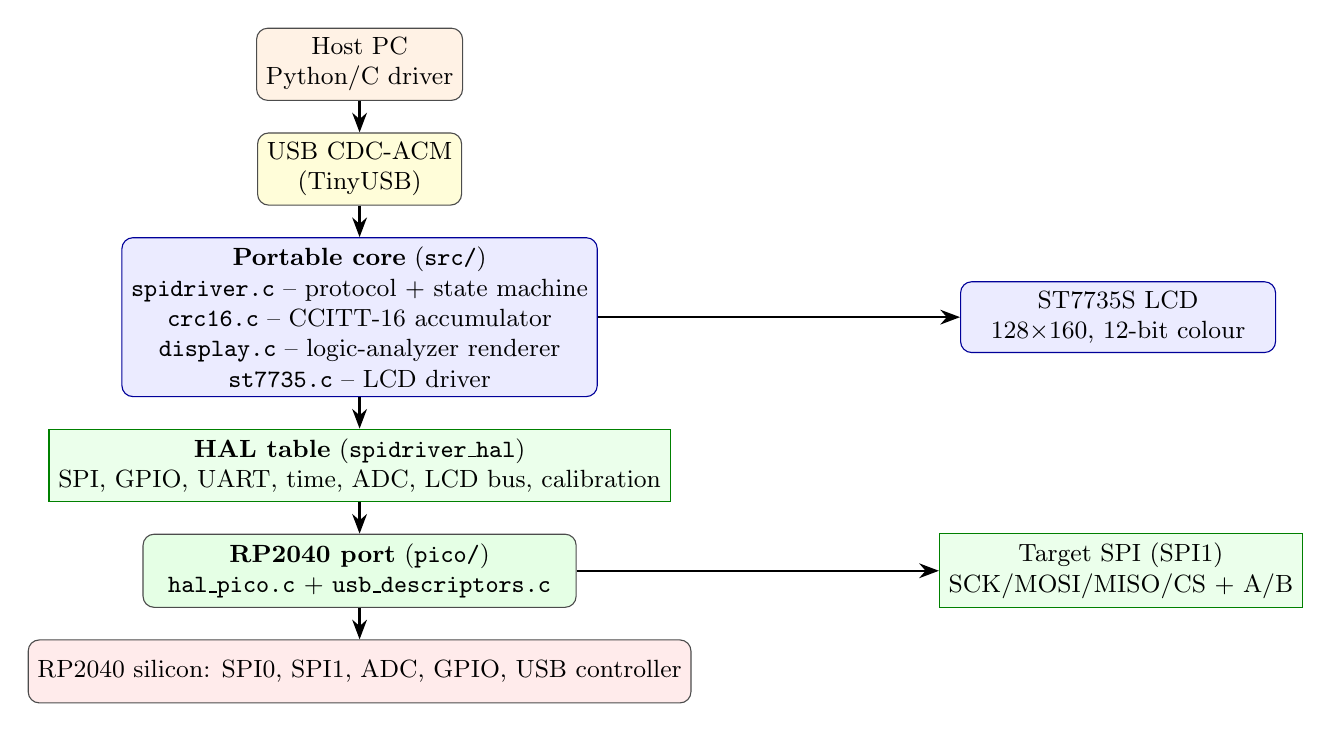
\begin{tikzpicture}[node distance=4mm]
  \node[block, fill=orange!10] (host) {Host PC\\ Python/C driver};

  \node[block, below=of host, fill=yellow!15] (usb) {USB CDC-ACM\\ (TinyUSB)};

  \node[blk, below=of usb, minimum width=55mm] (core) {
    \textbf{Portable core} (\texttt{src/})\\
    \texttt{spidriver.c} -- protocol + state machine\\
    \texttt{crc16.c} -- CCITT-16 accumulator\\
    \texttt{display.c} -- logic-analyzer renderer\\
    \texttt{st7735.c} -- LCD driver};

  \node[io, below=of core, minimum width=55mm] (hal) {
    \textbf{HAL table} (\texttt{spidriver\_hal})\\
    SPI, GPIO, UART, time, ADC, LCD bus, calibration};

  \node[block, below=of hal, fill=green!10, minimum width=55mm] (picohal) {
    \textbf{RP2040 port} (\texttt{pico/})\\
    \texttt{hal\_pico.c} + \texttt{usb\_descriptors.c}};

  \node[block, below=of picohal, fill=red!8] (hw) {
    RP2040 silicon: SPI0, SPI1, ADC, GPIO, USB controller};

  \draw[arr] (host) -- (usb);
  \draw[arr] (usb) -- (core);
  \draw[arr] (core) -- (hal);
  \draw[arr] (hal) -- (picohal);
  \draw[arr] (picohal) -- (hw);

  \node[blk, right=of core, xshift=42mm, minimum width=40mm] (disp) {
    ST7735S LCD\\ 128$\times$160, 12-bit colour};
  \node[io, right=of picohal, xshift=42mm, minimum width=40mm] (spi) {
    Target SPI (SPI1)\\ SCK/MOSI/MISO/CS + A/B};
  \draw[arr] (core) -- (disp);
  \draw[arr] (picohal) -- (spi);
\end{tikzpicture}
\caption{Layered architecture. The core is target-independent; only the HAL
  knows the RP2040.}
\label{fig:arch}
\end{figure}

\section{Pin map}

Both SPI buses are \emph{hardware} SPI (no bit-banging). The LCD rides
SPI0; the device-under-test rides SPI1. RP2040 hardware-SPI pins are fixed
per-function sets, which forces one compromise: target MOSI must land on
GP11 (physical pin~15) rather than the original board's pin~13.

\begin{table}[h!]
\centering
\begin{tabular}{@{}llll@{}}
\toprule
\textbf{Function} & \textbf{GPIO} & \textbf{Physical pin} & \textbf{Peripheral}\\
\midrule
LCD SCK  & GP2  & 4  & SPI0 SCK \\
LCD MOSI & GP3  & 5  & SPI0 TX \\
LCD DC   & GP4  & 6  & GPIO out \\
LCD CS   & GP5  & 7  & GPIO out \\
\midrule
Target SCK  & GP10 & 13 & SPI1 SCK \\
Target MOSI & GP11 & 15 & SPI1 TX \\
Target MISO & GP8  & 11 & SPI1 RX \\
Target CS   & GP9  & 12 & GPIO out \\
\midrule
Signal A    & GP6  & 9  & GPIO out \\
Signal B    & GP7  & 10 & GPIO out \\
\midrule
VBUS sense  & GP26 & -- & ADC0 \\
Current sense & GP27 & -- & ADC1 \\
Temperature & --   & -- & internal ADC4 \\
\bottomrule
\end{tabular}
\caption{RP2040 pin assignment. LCD RESET is tied to 3V3, as on the original
  board.}
\label{tab:pins}
\end{table}

The clock frequencies mirror the original: the LCD runs at 16\,MHz, the
target bus at 500\,kHz (the EFM8 clocked $\approx$490\,kHz). Both are
configurable via \texttt{SPI\_TARGET\_HZ}.

%=====================================================================
\section{USB CDC transport (TinyUSB)}
%=====================================================================

The original board used an FTDI UART bridge; the RP2040 replaces it with its
native USB controller and TinyUSB in device mode. The device enumerates as a
single CDC-ACM serial port.

\begin{table}[h!]
\centering
\begin{tabular}{@{}ll@{}}
\toprule
\textbf{Parameter} & \textbf{Value}\\
\midrule
VID/PID       & \texttt{2E8A:000A}\\
Class         & CDC-ACM (two interfaces: control + data)\\
Control EP    & \texttt{0x81} (8-byte)\\
Bulk OUT      & \texttt{0x02} (64-byte)\\
Bulk IN       & \texttt{0x82} (64-byte)\\
Serial string & derived from \texttt{pico\_get\_unique\_board\_id()}\\
RX/TX FIFO    & 256 bytes each\\
\bottomrule
\end{tabular}
\caption{USB descriptor summary.}
\label{tab:usb}
\end{table}

\subsection{Two correctness-critical details}

Two bugs surfaced during bring-up and shaped the final code:

\begin{enumerate}
\item \textbf{Interface count.} The configuration descriptor initially
  declared one interface, so the host never probed the CDC \emph{data}
  interface and the bulk endpoints were never instantiated. The fix is
  \texttt{USBD\_ITF\_MAX = 2} (control + data) inside
  \texttt{usb\_descriptors.c}.
\item \textbf{Explicit flush.} The bundled TinyUSB only auto-flushes the TX
  FIFO once 64 bytes are queued. Single-byte replies would sit in the FIFO
  indefinitely, so \texttt{uart\_put()} calls
  \texttt{tud\_cdc\_write\_flush()} after every byte.
\end{enumerate}

\subsection{1200-baud re-flash}

Opening the port at 1200\,baud reboots the chip into the RP2040 bootrom
(BOOTSEL), the same convention as \texttt{pico\_stdio\_usb} and Arduino:

\begin{lstlisting}[style=c]
void tud_cdc_line_coding_cb(uint8_t itf, cdc_line_coding_t const *line_coding) {
    (void)itf;
    if (line_coding->bit_rate == 1200) {
        reset_usb_boot(0, 0);
    }
}
\end{lstlisting}

This links \texttt{pico\_bootrom} and makes remote flashing button-free:
\texttt{stty -F /dev/ttyACM0 1200} drops the Pico into the mass-storage
bootrom, and a \texttt{.uf2} is copied in.

\subsection{RP2040 USB errata workaround}

The bundled TinyUSB gates a bulk-IN workaround for RP2040 errata
E5/E15 behind \texttt{TUD\_OPT\_RP2040\_USB\_DEVICE\_UFRAME\_FIX}, which no
one defines by default. Without it, an armed bulk-IN buffer can stop
answering IN tokens and the tail of a reply never reaches the host. The port
enables it in \texttt{tusb\_config.h}:

\begin{lstlisting}[style=c]
#define TUD_OPT_RP2040_USB_DEVICE_UFRAME_FIX 1
\end{lstlisting}

%=====================================================================
\section{Host protocol}
%=====================================================================

The byte-stream protocol is drop-in compatible with the original drivers.
Bytes are framed by count, not delimiters.

\begin{table}[h!]
\centering
\begin{tabular}{@{}lll@{}}
\toprule
\textbf{Command} & \textbf{Bytes} & \textbf{Effect}\\
\midrule
\texttt{?}        & 1        & transmit 80-byte status line\\
\texttt{e <b>}    & 2        & echo \texttt{<b>}\\
\texttt{s}        & 1        & select (CS low)\\
\texttt{u}        & 1        & unselect (CS high)\\
\texttt{a <b>}    & 2        & set A from bit~0 of \texttt{<b>}\\
\texttt{b <b>}    & 2        & set B from bit~0 of \texttt{<b>}\\
\texttt{x}        & 1        & disconnect (tri-state target bus)\\
\texttt{0x80--0xBF} & $1+n$  & duplex: clock $n$ bytes, echo $n$ MISO bytes\\
\texttt{0xC0--0xFF} & $1+n$  & write-only: clock $n$ bytes\\
\bottomrule
\end{tabular}
\caption{Command set. Transfer length $n = (\texttt{cmd} \,\&\, \texttt{0x3F})+1$.}
\label{tab:proto}
\end{table}

The status line is \emph{exactly} 80 bytes --- the host driver's
\texttt{getstatus} slices it blindly:

\begin{lstlisting}[style=proto]
[spidriver1 5303284740C3781C     48 1.928 322 31.2 0 0 1 0000]
\end{lstlisting}

Fields: product, serial, uptime~s, Vbus~V, current~mA, temperature~$^\circ$C,
A, B, CS, CRC-16.

%=====================================================================
\section{CRC-16}
%=====================================================================

The CRC is the CCITT-16 \emph{XMODEM} accumulator (polynomial 0x1021, initial
value 0). Every byte clocked out and every MISO byte clocked in is folded
into the accumulator. The status line reports the \emph{bit-reversed}
accumulator to match the original firmware:

\begin{lstlisting}[style=c]
uint16_t crc = crc16_bitreverse(st.crc);  // status reports this
\end{lstlisting}

%=====================================================================
\section{Measurements}
%=====================================================================

Three channels are sampled: Vbus (ADC0, via a divider), target current
(ADC1, via the ZXCT1110 current mirror on the original board), and the
internal temperature sensor (ADC4).

Each channel is read four times and box-averaged, then folded through an
exponential moving average with $\alpha=\tfrac18$, replicating the original
\texttt{ema} word:

\begin{equation}
  \text{new} = \frac{7\cdot\text{old} + \text{sample}}{8}
\end{equation}

All arithmetic is in ``raw16'' units, where $\text{raw16}=\text{raw12}\ll 4$
(a 12-bit ADC read left-shifted to 16 bits). Calibration constants are
scaled to raw16:

\begin{table}[h!]
\centering
\begin{tabular}{@{}lll@{}}
\toprule
\textbf{Constant} & \textbf{Value} & \textbf{Meaning}\\
\midrule
\texttt{cal\_vbus\_mv}    & 8250  & 3.3\,V ref, divider $V_\text{bus}=2.5\,V_\text{pin}$\\
\texttt{cal\_current\_ma} & 1375  & ZXCT1110, $R_s{=}0.1\,\Omega$, $R_g{=}2.4$k\\
\texttt{cal\_current\_zero} & 0    & offset subtracted before scaling\\
\texttt{cal\_temp\_coef}  & 19173 & RP2040 temp-sensor slope\\
\texttt{cal\_temp\_offset}& 4372  & deci-$^\circ$C at raw16 = 0\\
\bottomrule
\end{tabular}
\caption{Calibration constants (raw16 scale).}
\label{tab:cal}
\end{table}

%=====================================================================
\section{Main loop and concurrency}
%=====================================================================

Concurrency is deliberately simple. A 1\,ms repeating hardware timer fires
\texttt{spidriver\_tick()}, which advances the uptime counter and decrements
the slow-refresh counter. All other work happens in the foreground loop:

\begin{lstlisting}[style=c]
void spidriver_mainloop(spidriver_hal *hal) {
    for (;;) {
        conversions(hal);                 // ADC + EMA + scaling
        for (int i = 0; i < 64; i++) {    // drain command queue
            if (!spidriver_service(hal)) break;
        }
        if (st.dirty) {                   // waveform redraw
            st.dirty = false;
            display_waves(&st.lcd, st.history, st.hist_count, st.port);
        }
        if (st.slowc == 0) {              // 250 ms reading refresh
            st.slowc = 250;
            display_results(&st.lcd, st.vbus_mv, st.cur_ma);
        }
    }
}
\end{lstlisting}

The loop mirrors the original firmware's split between a background
measurement ``thread'' and a foreground command service.

%=====================================================================
\section{Logic-analyzer display}
%=====================================================================

The display renders six horizontal traces: SCK, MISO, MOSI, CS, A, B. A
14-entry history ring (the original's 42-byte ring) stores the most recent
bus events. Each event is tagged with a \emph{code} byte:

\begin{table}[h!]
\centering
\begin{tabular}{@{}lll@{}}
\toprule
\textbf{Code} & \textbf{Meaning} & \textbf{Width (columns)}\\
\midrule
\texttt{'a'} & port change (CS/A/B) & 18\\
\texttt{'b'} & write-only byte      & 18\\
\texttt{'c'} & duplex byte (MOSI$\rightarrow$MISO) & 18\\
\texttt{'d'} & disconnect           & 8\\
\bottomrule
\end{tabular}
\caption{Waveform entry codes and column widths.}
\label{tab:codes}
\end{table}

Rendering walks the history newest-first, right-to-left. Two key state
machines reconstruct the analogue signal:

\begin{itemize}
\item \textbf{MISO/MOSI} track a \emph{previous level} across byte
  boundaries, drawing a vertical edge whenever the last bit of one byte
  differs from the first bit of the next.
\item \textbf{CS/A/B} track the port state \emph{backward} through history:
  each \texttt{'a'} entry stores the port value \emph{before} the change, so
  walking right-to-left reconstructs the true signal level during every
  transfer.
\end{itemize}

Each byte is drawn as eight 2-pixel-wide bit cells (16 columns) plus a
trailing return-to-idle column, matching the original's 18-column byte cell.

\subsection{ST7735S driver}

The panel is 128$\times$160 in 12-bit colour. Two details matter:

\begin{enumerate}
\item \textbf{12-bit packing.} Pixels are 4-4-4 (BGR order) and packed
  two-per-three-bytes:
  \begin{equation}
    \underbrace{(b_0\ll4\,|\,g_0)}_{\text{byte 0}}\quad
    \underbrace{(r_0\ll4\,|\,b_1)}_{\text{byte 1}}\quad
    \underbrace{(g_1\ll4\,|\,r_1)}_{\text{byte 2}}
  \end{equation}
  The original naive port sent 16 bits per pixel, scrambling colours; the
  fix packs to three bytes per two pixels.
\item \textbf{Orientation.} Everything renders in literal portrait
  coordinates with \texttt{MADCTL = 0x08} (BGR). The original split text
  (0xC8) and waveform (0xA8) orientations; this port unifies them.
\end{enumerate}

\subsection{Fonts}

Two fonts are embedded, generated by \texttt{tools/genfonts.py}:

\begin{itemize}
\item \textbf{Micro} --- 4$\times$5 hexadecimal glyphs for the byte
  annotations under MISO/MOSI, nibble-packed (2 px/byte).
\item \textbf{Big} --- IBM Plex Sans SemiBold at 13\,pt, regenerated from
  the original face, 4-bit greyscale, nibble-packed. Digits are fixed
  8$\times$9. The generator crops glyphs from $y=5$ (the ink start for
  13\,pt Plex Sans); the original port cropped from $y=0$, which captured
  five blank rows and truncated the digit bottoms.
\end{itemize}

%=====================================================================
\section{Build}
%=====================================================================

\begin{lstlisting}[style=proto]
export PICO_SDK_PATH=/path/to/pico-sdk
cmake -B build
cmake --build build -j
# flash:
stty -F /dev/ttyACM0 1200        # reboot into BOOTSEL
udisksctl mount -b /dev/sdX1
cp build/spidriver_pico.uf2 /media/\$USER/RPI-RP2/
\end{lstlisting}

The core (\texttt{src/}) is shared with the POSIX host test target
(\texttt{host/}), so the protocol can be validated on a desktop without
hardware: \texttt{printf '?' | ./host/build/spidriver\_host} returns the
80-byte status line. A Python regression harness
(\texttt{host/test\_spidriver.py}) exercises status, echo, CS/A/B control,
duplex and write-only transfers, and a 100-round stress test over the real
USB link --- including full-raw tty handling (canonical mode and XON/XOFF
would otherwise swallow reply bytes).

\end{document}
